\documentclass[draft=false
              ,paper=a4
              ,twoside=false
              ,fontsize=11pt
              ,headsepline
              ,BCOR10mm
              ,DIV11
              ]{scrbook}
\usepackage[ngerman,english]{babel}
\usepackage[T1]{fontenc}
\usepackage[utf8]{inputenc}
\usepackage{libertine}
\usepackage{pifont}
\usepackage{microtype}
\usepackage{textcomp}
\usepackage[german,refpage]{nomencl}
\usepackage{setspace}
\usepackage{makeidx}
\usepackage{listings}
\usepackage{natbib}
\usepackage[ngerman,colorlinks=true]{hyperref}
\usepackage{soul}
\usepackage{hawstyle}

%% define some colors
\colorlet{BackgroundColor}{gray!20}
\colorlet{KeywordColor}{blue}
\colorlet{CommentColor}{black!60}
%% for tables
\colorlet{HeadColor}{gray!60}
\colorlet{Color1}{blue!10}
\colorlet{Color2}{white}

%% configure colors
\HAWifprinter{
  \colorlet{BackgroundColor}{gray!20}
  \colorlet{KeywordColor}{black}
  \colorlet{CommentColor}{gray}
  % for tables
  \colorlet{HeadColor}{gray!60}
  \colorlet{Color1}{gray!40}
  \colorlet{Color2}{white}
}{}
\lstset{%
  numbers=left,
  numberstyle=\tiny,
  stepnumber=1,
  numbersep=5pt,
  basicstyle=\ttfamily\small,
  keywordstyle=\color{KeywordColor}\bfseries,
  identifierstyle=\color{black},
  commentstyle=\color{CommentColor},
  backgroundcolor=\color{BackgroundColor},
  captionpos=b,
  fontadjust=true
}
\lstset{escapeinside={(*@}{@*)}, % used to enter latex code inside listings
        morekeywords={uint32_t, int32_t}
}
\ifpdfoutput{
  \hypersetup{bookmarksopen=false,bookmarksnumbered,linktocpage}
}{}

%% more fancy C++
\DeclareRobustCommand{\cxx}{C\raisebox{0.25ex}{{\scriptsize +\kern-0.25ex +}}}

\clubpenalty=10000
\widowpenalty=10000
\displaywidowpenalty=10000

% unknown hyphenations
\hyphenation{
}

%% recalculate text area
\typearea[current]{last}

%% no indentation at paragraphs
\setlength\parindent{0pt}
\setlength\parskip{\medskipamount}

\makeindex
\makenomenclature

\begin{document}
\selectlanguage{ngerman}

%%%%%
%% customize (see readme.pdf for supported values)
\HAWThesisProperties{Author={Daniel Schruhl}
                    ,Title={Entwurf und Implementierung einer STDMA Station}
                    ,EnglishTitle={Design and implementation of an STDMA station}
                    ,ThesisType={Referat}
                    ,ExaminationType={Referat eingereicht im Rahmen der Vorlesung Verteilte Systeme}
                    ,DegreeProgramme={Angewandte Informatik (AI)}
                    ,ThesisExperts={Prof. Dr. C. Klauck}
                    ,ReleaseDate={31. Mai 2017}
                  }

%% title
\frontmatter

%% output title page
\maketitle

\onehalfspacing

%% add abstract pages
%% note: this is one command on multiple lines
\HAWAbstractPage
%% German abstract
{STDMA, Verteilte Systeme, Clojure}%
%% English abstract
{STDMA, Distributed Systems, Clojure}%

\newpage
\singlespacing

\tableofcontents
\newpage
%% enable if these lists should be shown on their own page
%%\listoftables
%%\listoffigures
\lstlistoflistings

%% main
\mainmatter
\onehalfspacing
%% write to the log/stdout
\typeout{===== File: chapter 1}
%% include chapter file (chapter1.tex)
%%\include{chapter1}

\chapter{Einführung und Ziele}
In verteilten Systemen werden oft Nachrichten unter verschiedenen Teilnehmern eines Netzes ausgetauscht. Dabei sind diese Teilnehmer oft nur durch ein Medium miteinander verbunden. Dieses eine Medium muss dann mehrere Teilnehmer unterstützen können.

Um dieses Problem zu lösen soll ein Softwareprodukt erstellt werden, das eine Station darstellt, die auf einem Medium Nachrichten empfangen und senden kann.

Dabei sollen mehrere Stationen auf einem Medium Nachrichten verschicken und senden. Das geschieht, indem das Medium in feste Frames aufgeteilt wird und jeder Frame eine feste Anzahl an Slots hat, in dem aus allen teilnehmenden Stationen immer nur eine in ihrem zugeteilten Slot Senden darf. Das Medium wird hierbei im Betracht der Zeit aufgeteilt. Diese Aufteilung (Multiplexing) wird auch time-division multiple access (TDMA) genannt.
In diesem Fall sollen die Stationen selber untereinander ihre Slots zum Senden verwalten und untereinander gleichmäßig aufteilen.
Das wird auch Self-organized time-division multiple access (STDMA) genannt.

\section{Randbedingungen}
Das zu verwendende Medium ist ein Socket, der per IP Multicast Nachrichtenpakete (Datagrams) an mehrere Klienten austeilen kann. Die TTL der Multicast-Pakete ist auf 1 zu setzen, um unnötige Netzlasten und Netzstörungen zu vermeiden.

Die Frames haben eine Länge von einer Sekunde. Ein Frame hat 25 Slots. Diese sind von 1 bis 25 nummeriert. Die Frames sind in
Sekunden seit dem 1.1.1970, 00:00 Uhr nummeriert.

\begin{figure}[h]
\centering
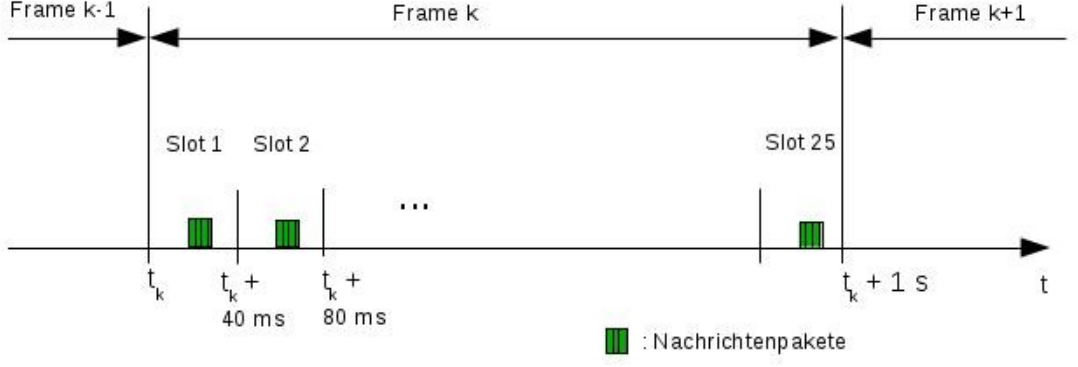
\includegraphics[width=\textwidth]{frame-structure.png}
\caption[frame-structure]{Aufteilung des Mediums in Frames und Slots, Quelle: \cite{exercise}}
\label{fig:frame-structure}
\end{figure}

Jede Station darf nur einmal pro Frame senden. Das muss in der Mitte ihres zugeteilten Slots passieren.

Die Vergabe der Slots soll ohne zentrale Vergabeinstanz geschehen. Das geschieht, indem jedes Nachrichtenpaket ein Datenfeld enthält, in das die sendende Station die Nummer ihres Slots einträgt, die sie für den nächsten Frame zum Senden verwendet.
Das bedeutet also, dass durch das Lesen der Nachrichtenpakete in einem Frame bestimmt werden kann, welche Slots im nächsten Frame frei sind.

Ein Nachrichtenpaket hat folgende Struktur:
\begin{itemize}
	\item Byte 0: Stationsklasse ('A' oder 'B')
	\item Byte 1 – 24: Nutzdaten. (Darin Byte 1 – 10: Name der sendenden Station.)
	\item Byte 25: Nummer des Slots, in dem die Station im nächsten Frame senden wird.
	\item Byte 26 – 33: Zeitpunkt, zu dem dieses Paket gesendet wurde. Einheit: Millisekunden seit dem 1.1.1970 als 8-Byte Integer, Big Endian.
\end{itemize}

Gesamtlänge: 34 Bytes

Stationen haben dabei eine Unterteilung in Klasse A und B. Diese Klassen werden für eine Synchronisierung der Zeit verwendet. Generell wird die UTC Zeit verwendet. Die Uhr einer Station kann einen anfänglichen Offset haben. Die Stationen synchronisieren dann untereinander im Laufe der Teilnahme am Netz ihre Uhren untereinander, so dass der Offset sich verändern kann.

Klasse A Uhren gelten als hinreichend genau und als Referenz zur Synchronisation. Klasse B und Klasse A Stationen können dann anhand anderer empfangen Nachrichtenpakete von Klasse A Stationen ihren Offset verändern. Dabei wird die Sendezeit und die Klasse innerhalb eines Nachrichtenpaketes verwendet.

Bei Kollisionen sollen die betroffenen Nachrichtenpakete als nicht empfangen betrachtet werden. Ein kollisionsfreier Betrieb mit maximal 25 Stationen muss nach endlicher Zeit erreicht werden und darf nicht wieder verlassen werden.

Das Produkt soll über die Kommandozeile gestartet werden können. Dabei müssen folgende Parameter mit übergeben werden können:
\begin{itemize}
	\item Interfacename des Kommunikationsendpunktes
	\item Adresse der Multicast Gruppe, Klasse D IP-Adresse
	\item Port des Sockets
	\item Stationsklasse, A oder B
	\item Anfänglicher UTC Offset
\end{itemize}
Als Datenquelle für die Nutzdaten soll das STDIN des Produktes verwendet werden, um der Station neue Nutzdaten zukommen zu lassen.

\section{Kontextabgrezung}
Das Produkt muss auch in einer ssh-Sitzung auf einem anderen Rechner gestartet werden können. Es muss auf Rechnern mit Linux Betriebssystem lauffähig sein.

\chapter{Gesamtsystem}
Das Produkt ist in Clojure (v1.9) umgesetzt worden. Clojure ist eine funktionale Programmiersprache, die auf der JVM läuft. Dabei ist eine interoperabilität mit Java möglich. Das erleichtert den Umgang mit Sockets, da der Umgang mit diesen in Java gut dokumentiert und verwendbar ist. Außerdem hat Clojure im Vergleich mit Erlang einige andere Vorteile wie lazily evaluated Sequences oder eine bessere Testumgebung.

Funktionale Programmiersprachen haben den Vorteil in verteilten Systemen, das die Ergebnisse von Funktionen bei gleichen Parametern immer gleich sind. Diese Immutability von Daten hat den Vorteil, das nebenläufige Prozesse dadurch keine Datensynchronisation machen müssen. Dadurch wird eine erhöhte Threadsicherheit erreicht.

\section{Architekturüberblick}

\section{Konfigurationsparameter}

\section{Benutzungsschnittstellen}

\chapter{Subsysteme und Komponenten}

\section{Connector}

\subsection{Aufgabe und Verantwortung}

\subsection{Schnittstelle}

\subsection{Entwurfsentscheidungen}

\subsection{Konfigurationsparameter}

\section{Payload-Source}

\subsection{Aufgabe und Verantwortung}

\subsection{Schnittstelle}

\subsection{Entwurfsentscheidungen}

\subsection{Konfigurationsparameter}

\section{Message-Writer}

\subsection{Aufgabe und Verantwortung}

\subsection{Schnittstelle}

\subsection{Entwurfsentscheidungen}

\subsection{Konfigurationsparameter}

\section{Station}

\subsection{Aufgabe und Verantwortung}

\subsection{Schnittstelle}

\subsection{Entwurfsentscheidungen}

\subsection{Konfigurationsparameter}


%% appendix if used
%%\appendix
%%\typeout{===== File: appendix}
%%\include{appendix}

% bibliography and other stuff
\backmatter

\typeout{===== Section: literature}
%% read the documentation for customizing the style
\bibliographystyle{dinat}
\bibliography{documentation}

\typeout{===== Section: nomenclature}
%% uncomment if a TOC entry is needed
%%\addcontentsline{toc}{chapter}{Glossar}
\renewcommand{\nomname}{Glossar}
\clearpage
\markboth{\nomname}{\nomname} %% see nomencl doc, page 9, section 4.1
\printnomenclature

%% index
\typeout{===== Section: index}
\printindex
\chapter{Erklärung zur schriftlichen Ausarbeitung des Referates}
\HAWasurency

\end{document}
